\section{Evaluation}
\label{sec:evaluation}

\subsection{Methodology and provenance}
\label{sec:eval_setup}

The evaluation answers five research questions:
\begin{itemize}
  \item \textbf{RQ1: Correctness.} Does the implemented authenticated format preserve nonce/generation, publication, and metadata-authentication invariants under retained remount, fault, and tamper campaigns?
  \item \textbf{RQ2: Mode-aligned baselines.} What cost does AEGIS-Q impose relative to retained plaintext and gocryptfs rows under the frozen filesystem contract?
  \item \textbf{RQ3: QoS/hero result.} Does AEGIS-Q recover foreground SQLite latency under mounted secure-storage pressure relative to unthrottled pressure and a simple controller?
  \item \textbf{RQ4: Freshness and recovery.} What oracle-classified recovery and TPM-freshness outcomes are supported by the retained fault campaigns?
  \item \textbf{RQ5: Ablation and sensitivity.} Which mechanisms account for the measured placement, controller, key-plane, and anchor behavior, and how sensitive is the SQLite controller?
\end{itemize}

The design/evaluation contract is one closure per main mechanism: authenticated block format closes through the generation/tamper evidence in RQ1; D/J/C publication closes through oracle-labeled daemon/app cut points in RQ4; CPU/GPU placement closes through the data-plane and key-plane measurements in RQ2/RQ5; TPM freshness closes through the hardware-freshness matrix in RQ4; the QoS controller closes through SQLite recovery and sensitivity traces in RQ3/RQ5; and the optional ML-KEM lane closes through the mounted open-file rekey workflow in RQ5.

Primitive-placement numbers come from the verified microbenchmark harness; the mounted rekey result comes from the key-plane workflow harness.  Both capture provenance and refuse to manufacture unsupported configurations.  The completeness gate keeps baseline cost, mounted pressure, workload diversity, placement breakdown, sensitivity, stability limits, and the SQLite case study retained while leaving missing kernel rows and statistical generalization to Discussion.

The platform was an NVIDIA Jetson AGX Thor Developer Kit with 14 ARM CPU cores, a 1~TB WD PC SN5000S NVMe device, Linux~6.8.12-tegra, CUDA~13.0.48, liboqs~0.15.0, FUSE3~3.14.0, and the cuPQC libraries found by CMake.  The result is not an Orin Nano result and must not be generalized to other Jetson generations.  The current evidence has three tiers: Figure~\ref{fig:baseline_comparison} is a diagnostic placement result with three repetitions and observed-range whiskers, not confidence intervals; the key-plane and SQLite bundles are single retained workflow artifacts, not statistical confidence claims; future headline comparisons require warmup, five repetitions, bootstrap 95\% confidence intervals, outlier policy, fixed governor/clock/power capture, thermal logs, background-process control, cache policy, and fail-closed handling for missing logs or failed modes.

Table~\ref{tab:benchmark_workloads} states what each experiment can and cannot establish.  The v2 filesystem contract fixes 4~KiB 70/30 random read/write, \texttt{psync}, per-write \texttt{fdatasync}, warm/cold cache policy, queue depth~1, one client, a sparse-prepared 1~GiB file, fixed mounts/platform, five repetitions, and bootstrap 95\% confidence intervals.  The plaintext warm-cache row reports 32.88~MiB/s median throughput and 0.165~ms conservative p99 (95\% CIs 30.16--36.96 and 0.157--0.167); gocryptfs reports 21.72~MiB/s and 0.060~ms (21.19--21.86 and 0.0596--0.0622); the AEGIS-Q warm-cache row reports 0.359~MiB/s and 11.21~ms (0.286--0.547 and 7.70--13.70).  The mechanism-ablation manifest uses these rows to gate the format gap and links the controller, key-plane, and anchor variants to the RQ5 evidence below; broader kernel-encryption rows are discussed in Section~\ref{sec:disc_roadmap}.

\begin{table}[t]
\centering
\caption{Evaluation scope by research question.}
\scriptsize
\setlength{\tabcolsep}{2pt}
\begin{tabularx}{\columnwidth}{P{0.25\columnwidth}|Y|Y}
\toprule
\textbf{RQ / exp.} & \textbf{Establishes} & \textbf{Does not establish}\\
\midrule
RQ1 FUSE & Format functions after clean remount & Full SQLite/crash certification\\
RQ1 hash & CUDA and OpenSSL digests agree & Side-channel resistance\\
RQ2 Frozen contract & Plaintext, gocryptfs, and AEGIS-Q warm rows & fscrypt/dm-crypt and cold rows\\
RQ2/RQ5 UMA & Managed allocation and host/device prefetch complete & Verified storage-DMA or O\_DIRECT-to-UVM\\
RQ2/RQ5 eBPF & \texttt{nvme\_complete\_rq} histogram retained & Mounted eBPF/io\_uring path\\
RQ3 daemon & Scheduler prototype and telemetry scripts exist & End-to-end AI p99 controller\\
RQ3 stress & 4-writer tail-latency probe under pressure & End-to-end AI workload\\
RQ3 TensorRT & Interference traces and samples are retained & Closed-loop QoS controller\\
RQ4 file anchor & File snapshot rollback remains visible & TPM-anchor freshness\\
\bottomrule
\end{tabularx}
\label{tab:benchmark_workloads}
\end{table}

\subsection{CPU for bulk data, GPU for batched ML-KEM}
\label{sec:eval_performance}

Figure~\ref{fig:baseline_comparison} reports the diagnostic placement result.  For a 16~MiB AES-256-GCM input, CPU/OpenSSL reaches 1.61~GB/s (observed 1.59--1.63~GB/s), whereas the managed-buffer GPU path reaches 0.172~GB/s (0.172--0.172~GB/s).  The GPU result includes managed-buffer staging and stream synchronization.  Smaller requests amplify the same effect.  This is why AEGIS-Q's data plane is CPU-first; a GPU label alone is not a performance result.

For a batch of 4,096 ML-KEM-768 key generations, liboqs on CPU reaches 64.8~K operations/s (64.3--64.9~K), while cuPQC reaches 1.50~M operations/s (1.49--1.51~M), a 23.2$\times$ ratio of medians.  The comparison is a primitive microbenchmark on one platform, not a claim that a FUSE write becomes 23.2$\times$ faster.  It supports the narrower policy of reserving GPU work for sufficiently large, independent key-plane batches.

The retained mounted ML-KEM-768 key-plane workflow opens 1,024 encrypted files and refreshes their HMAC-authenticated envelopes.  CPU-only refresh takes 24.399~ms (41,969.6 files/s).  With explicit slack, admission selects the GPU and finishes in 21.070~ms (48,599.0 files/s), a 1.158$\times$ speedup.  With zero slack and high memory-pressure telemetry, admission falls back to CPU in 24.411~ms with an AI-QoS-exhausted deferral.  This supports only maintenance-visible open-file envelope refresh, not hardware-backed credential release, a persistent KEM hierarchy, or foreground AI QoS recovery.

These measurements produce the main placement rule used by the design: AES-GCM data writes are latency-sensitive and remain CPU-first, while ML-KEM batches are elastic and may use the GPU only when producer slack and telemetry permit it.  The result would be weaker if the paper reported only the faster GPU primitive; the important systems observation is the asymmetry between the data plane and the batch plane.

\begin{figure*}[t]
  \centering
  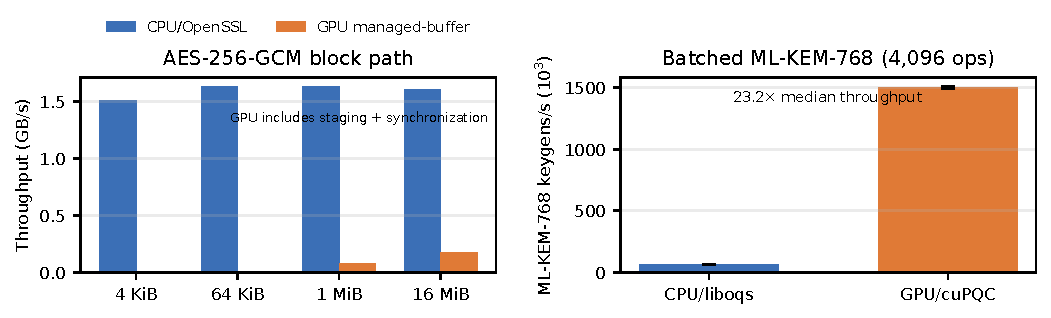
\includegraphics[width=0.94\textwidth]{Figures/fig_verified_microbench.pdf}
  \caption{Placement result for RQ2/RQ5. CPU AES-GCM exceeds managed-buffer GPU for the data plane; cuPQC improves batched ML-KEM-768. Bars are medians with observed 5th--95th-percentile whiskers.}
  \Description{Two bar charts generated from three raw benchmark runs. The first shows CPU AES-GCM throughput exceeding the managed-buffer GPU path. The second shows GPU cuPQC ML-KEM key generation exceeding the CPU liboqs result for a batch of 4,096.}
  \label{fig:baseline_comparison}
\end{figure*}

\subsection{Correctness and negative controls}
\label{sec:eval_workloads}

The GPU integrity test passes leaf, Merkle, and empty-tree parity cases against OpenSSL.  The FUSE self-test passes journal/checkpoint/anchor unit checks and a generation-replay regression: appending an older generation after a newer mapping does not supersede the newer mapping, and decrypting a generation-2 ciphertext/tag under generation~1 fails.  The retained generation fault matrix then runs the final FUSE binary through partial update, clean remount, torn journal tail, stale snapshot replay, and adversarial older-generation append cases.  Its parsed journals show no duplicate generated \((\mathit{block},\mathit{generation})\) pairs; every trial receives an explicit oracle verdict, with no silent-corruption or unexpected-liveness verdict.  The clean-remount regression writes 128~KiB, calls \texttt{fsync}, remounts, byte-compares plaintext, and verifies that the sidecar does not contain the complete input sequence.  A separate final-binary test flips the persisted HMAC-authenticated envelopes and observes \texttt{EKEYREJECTED}.  These results strengthen the generation and envelope claims; the daemon matrix below supplies the selected daemon-crash evidence.

The POSIX-scope audit records the narrow interface: default encrypted-file \texttt{mmap} fails with \texttt{ENODEV}; disjoint writers recover the expected blocks; rename and directory \texttt{fsync} return \texttt{ENOTSUP}; user xattrs round-trip while internal xattrs are hidden; writeback-cache/direct-IO mmap capabilities are not requested; and lower-filesystem xattr atomicity and directory durability remain delegated.

Auxiliary storage/GPU diagnostics are deliberately scoped.  The retained host-pinning and managed-storage probes show same-buffer CPU/GPU checksum agreement plus CUDA pointer diagnostics, but they do not prove UVM migration suppression or final FUSE data-path DMA.

The file-backed anchor produces the deliberately negative result: restoring an entire backing-directory snapshot is classified as \texttt{rollback\_visible}, i.e., the previous committed baseline remains readable.  The result remains a negative control rather than rollback resistance.

The TPM artifacts record anchor latency, fixed properties, PCR reads, NV public attributes for index \texttt{0x01500010}, and a transient PCR-policy probe that unseals under the current PCR digest but rejects a drifted digest.  The hardware-freshness recovery matrix gives explicit oracle verdicts for stale disk/new TPM, new disk/stale TPM, missing index, changed PCRs, authorization failure, interrupted NV update, and normal replay-after-advance.  The real-TPM rows cover replay, missing index, changed-PCR probe behavior, and wrong authorization; the new-disk/stale-TPM and interrupted-update rows are final-binary command-path fault injection, not physical power-loss evidence.  This is replay-after-advance evidence, not a claim that the persistent filesystem anchor itself is PCR-sealed.

The broader crash/replay matrices are selected-boundary regression evidence, not complete app-level crash coverage.  The daemon power-fault campaign kills the final binary at one-block data write, journal append/fsync, logical-size/checkpoint xattr, anchor update, \texttt{fsync}, remount-validation, and authenticated-read cut points; all nine rows retain a marker, daemon \texttt{SIGKILL}, and an acceptable oracle verdict.  The same manifest ties application-level commit coverage to 20 SQLite WAL/FULL selected-boundary trials, three SQLite DELETE/EXTRA \texttt{fdatasync} app-crash trials, and a \texttt{dbm.dumb} TPM replay row; a separate audit finds no unclassified retained recovery row.  This is selected daemon/app evidence, not physical power-loss, kernel-crash, drive-cache, arbitrary-workload, or multi-block raw-write atomicity certification.

Table~\ref{tab:recovery_scope} summarizes the interpretation and the next experiment required to strengthen each row.

\begin{table}[t]
\centering
\caption{Recovery/freshness outcomes and their interpretation.}
\scriptsize
\setlength{\tabcolsep}{3pt}
\begin{tabularx}{\columnwidth}{P{0.28\columnwidth}|P{0.30\columnwidth}|Y}
\toprule
\textbf{Retained result} & \textbf{Interpretation} & \textbf{Still missing}\\
\midrule
Clean FUSE remount & Envelope/key hierarchy can recover the written file after clean unmount/remount & Crash timing across all D/J/C boundaries\\
Metadata HMAC tamper & Unauthenticated envelope metadata fails closed & Full ciphertext/journal tamper campaign\\
File-anchor replay visible & File-backed witness is a negative control & External freshness state\\
TPM replay-after-advance fail closed & Current provisioned NV index can reject stale disk state after anchor advance & Persistent PCR policy and lifecycle\\
Daemon/app fault matrix & Retained daemon and SQLite/\texttt{dbm.dumb} cut points recover to acceptable oracle states & Physical power loss, drive caches, and broader workloads\\
SQLite/\texttt{dbm.dumb} stale snapshots & Two workloads fail closed on TPM-backed stale replay & Broader workload matrix\\
\bottomrule
\end{tabularx}
\label{tab:recovery_scope}
\end{table}

\subsection{QoS Recovery, Ablations, and Sensitivity}
\label{sec:eval_qos}

Retained tegrastats/CUPTI artifacts show platform pressure reaching the mounted daemon: they record 8 and 5 daemon-throttled flushes, respectively.  This remains wiring evidence rather than TensorRT/AI p99 recovery or fast-notification bypass.

The app-level result uses SQLite transaction latency as the foreground workload.  Table~\ref{tab:qos_sqlite_recovery} is generated from the retained four-mode bundle.  Mounted storage pressure raises SQLite p99 from 6.4~ms to 13.8~ms and causes one 10~ms deadline miss.  AEGIS-Q marks foreground files latency-sensitive, throttles only elastic background writes, and recovers to 8.8~ms p99 with no misses at 2.7~MB/s.  The simple controller reaches 8.2~ms p99 at 2.3~MB/s.  This is SQLite recovery, not general AI-inference QoS.

The sensitivity bundle varies budget, sampling interval, threshold, queue depth, and writer intensity.  Its baseline p99 is 6.4~ms; 80~ms sampling and 128~KiB chunks remain at 7.0/7.2~ms, high threshold disables throttling (0 sleeps, 8.8~ms), and two writers is fragile (12.3~ms, one miss).  No-throttle and no-slack fallbacks pass, and the scripted hysteresis trace records 9 transitions and 8 flips.

Together, the ablation rows attribute observed behavior to four mechanisms: the authenticated FUSE format accounts for the warm-cache filesystem cost, elastic-write throttling accounts for SQLite p99 recovery, the GPU lane helps only the mounted open-file key refresh workflow with slack, and the TPM anchor converts the file-anchor replay negative control into fail-closed replay-after-advance behavior.  The sensitivity sweep then tests whether the QoS result depends on one constant rather than a stable controller regime.

\begin{table}[t]
\centering
\caption{SQLite p99 under mounted secure-storage pressure.  Hero rows are five-run medians; kernel rows are 3 retained runs each.}
\scriptsize
\setlength{\tabcolsep}{2pt}
\begin{tabularx}{\columnwidth}{P{0.18\columnwidth}|P{0.22\columnwidth}|r|r|r|P{0.18\columnwidth}}
\toprule
\textbf{Row} & \textbf{Control} & \textbf{p99} & \textbf{Miss} & \textbf{MB/s} & \textbf{Evidence}\\
\midrule
App only & none & 7.25 & 0.00 & 0.00 & 5-run med.\\
Unthrottled & none & 9.62 & 0.00 & 6.98 & 5-run med.\\
Simple ctrl. & harness sleep & 7.54 & 0.00 & 1.50 & 5-run med.\\
AEGIS-Q & storage class & 8.15 & 0.00 & 3.02 & 5-run med.\\
Kernel ionice & \texttt{ionice -c 3} & 16.22 & 6.00 & 7.25 & 3-run proof\\
Kernel IOWeight & \texttt{IOWeight=10} & 12.57 & 7.00 & 6.73 & 3-run proof\\
\bottomrule
\end{tabularx}
\label{tab:qos_sqlite_recovery}
\end{table}

